\documentclass[fleqn, 12pt]{article}
\usepackage[T1]{fontenc}
\usepackage{tocloft}
\usepackage[margin=1.1in]{geometry} 
\usepackage{amsmath,amsthm,amssymb,amsfonts, fancyhdr, color, comment, graphicx, environ}
\usepackage{xcolor}
\usepackage{mdframed}
\usepackage{graphicx}
\usepackage{caption}
\usepackage{subcaption}
\usepackage[shortlabels]{enumitem}
\usepackage{indentfirst}
\usepackage{hyperref}
\usepackage[serbian]{babel}
\renewcommand{\footrulewidth}{1 pt}
\usepackage{cite}
\bibliographystyle{plain}
\usepackage{float}

\hypersetup{
    colorlinks=true,
    linkcolor=blue,
    filecolor=magenta,      
    urlcolor=blue,
}


\pagestyle{fancy}



\newenvironment{problem}[2][Problem]
    { \begin{mdframed}[backgroundcolor=gray!20] \textbf{#1 #2} \\}
    {  \end{mdframed}}


\newenvironment{solution}{\textbf{Solution}}


\lhead{Mitar Avramović}
\rhead{Računarstvo i društvo} 
\chead{\textbf{}}
\lfoot{Doc. dr Sana Stojanović Đurđević}
\rfoot{Matematički fakultet, Beograd}

\renewcommand{\contentsname}{Sadržaj}
\begin{document}
\title{\Large Kurs: Računarstvo i društvo  \\[0.5cm]
        \bf\Large Bezbednost naših lozinki}
\author{\large Autor: Aleksa Jovanović\\ \ \\}
\date{\large Datum: \today}

\makeatletter
    \begin{titlepage}
        \begin{center}
	    {\ \\ \ \\}
        \vbox{}\vspace{5cm}
            {\@title }\\[3cm] 
            {\@author}
            {\large Predmetni profesor: \bf Prof. Sana Stojanović Đurđević\\  \ \\}
            {\@date\\}

        \end{center}
    \end{titlepage}
\makeatother
\setcounter{tocdepth}{2}
\tableofcontents
\newpage
\section{Uvod}
Pre svega, pozabavićemo se formalnom definicijom OSINT-a, kao i njegovim istorijskim začecima. Kasnije ćemo videti koliko se razvoj Interneta odrazio na porast kako resursa, tako i korišćenja OSINT istraga. 

\subsection{Definicija}\
Termin Open Source Intelligence (OSINT) se pre svega odnosi na specifičan izvor saznanja. Uopšteno, izvori saznanja se koriste za stvaranje sirovih podataka koji mogu biti procesuirani u šest koraka obrade podataka za stvaranje uvida. Open Source Intelligence se definiše kao \textbf{skup podataka stvoren iz javno dostupnih izvora} koji je prikupljen i obrađen za odgovarajuću publiku za potrebe davanja odgovora na specifično pitanje.

\subsection{Istorija}
U modernoj eri, OSINT je postao posebno važan tokom Drugog svetskog rata. Jedna od ključnih figura u razvoju OSINT-a bio je Vilijam Donovan, osnivač Odeljenja za strateške usluge (OSS). Unutar OSS-a, čitav jedan deo je bio posvećen analizi javno dostupnih informacija u obliku prikupljanih novina kao i radio prenosa širom sveta, držeći se reči svog osnivača „čak i režimski mediji će izdati nacionalne interese u očima neumornog posmatrača“. OSS je koristio novine, časopise, radio prenose i druge javno dostupne izvore kako bi prikupio informacije o neprijateljima i njihovim aktivnostima. OSS je koristio te informacije za analizu političkih, ekonomskih i vojnih trendova, što je doprinelo donošenju informisanih odluka tokom rata. \newline


Nakon Drugog svetskog rata, OSS je rasformiran, ali je njegova funkcija preuzeta od strane novoformirane Centralne informativne agencije (CIA). CIA je nastavila da koristi OSINT istrage kao deo svojih obaveštajnih aktivnosti. Tokom Hladnog rata, OSINT istrage postaju još važnije, jer su informacije iz javnih izvora bile ključne za praćenje aktivnosti Sovjetskog Saveza i drugih komunističkih zemalja. U isto vreme, druge zemlje su takođe razvijale svoje kapacitete za OSINT istrage. Na primer, britanska obaveštajna služba MI6 i sovjetski KGB su koristili otvorene izvore za prikupljanje informacija.
\newpage
\subsection{Internet}
Porastom upotrebe interneta se priroda javnih informacija menja u korenu. Čak i novine su sve više prisutne u digitalnom svetu, sa čestim ažuriranjem. Ovo rezultira bržim i lakšim pristupom novostima. Dodatno, internet pruža još više opcija svakom svom korisniku za iskazivanje vesti, znanja i mišljenja sa minimalnim, gotovo nepostojanim restrikcijama. Ovo je ojačano raznovrsnošću novih javnih izvora poput ličnih sajtova, foruma, blogova, društvenih mreža itd. Takođe, razne kompanije i organizacije koriste priliku da daju informacije i nude usluge poput pretraživača, platformi za društvene mreže, platformi za trgovinu, sajtova za upoznavanje itd.\newline

Ove usluge se koriste i ohrabruju korisnike da dele širok spektar ličnih informacija koje se vezuju za online pseudonim, ili u nekim situacijama čak i lična imena. Trend davanja osetne količine ličnih informacija je relativno nov, sve više prisutan od omasovljavnja društvenih mreža krajem prve decenije novog milenijuma.  To se može videti kao jaka suprotnost incidentu iz 1983. godine u Nemačkoj kada su zbog zahteva za neke lične informacije za potrebe novouvedenog popisa stanovništva izbili masovni protesti.
Iako je do nekih malo teže doći, većina izvora se smatra javno dostupnim. Prisutnost izvora na internetu se može kretati od svega nekoliko godina do više od jedne decenije.\newline

Ono što nam ostaje kao posledica sve većeg prisustva interneta i njegovih usluga u našim životima je da svi ovi izvori informacija nisu dostupni samo ljudima i organizacijama koje se bave obaveštajnim poslom. Iz raznoraznih razloga, veliki broj raznih lica i organizacija razvija i koristi alate i tehnike kako bi analizirali javno dostupan sadržaj.
\newpage
\section{Upotrebe OSINT-a}
Kao što je navedeno u prvom delu, ovde ćemo se pozabaviti širokim spektrom upotrebe OSINT-a. Primeri upotrebe koji se mogu naći se kreću od vojnih do civilnih, od krajnje dobronamernih do malicioznih.\newline

\textbf{Vojno-obaveštajne službe}: 2015. godine u junu, jedan džihadista ISIL-a kači selfi koji u pozadini sadrži fabriku bombi u Siriji. Korišćenjem geolokacijskih podataka sa slike, 23 sata kasnije, SAD napada i uništava tu istu fabriku.\newline

\textbf{Novinarstvo}: Belingketski kolektiv (koji uključuje istraživače, inspektore i amaterske novinare) predstavlja organizaciju koja prevashodno koristi javne izvore i društvene mreže za svoja istraživanja. Oni su uspeli da povežu ruske obaveštajce sa istragom Leta 17 Malasiya Airlines-a kao i trovanjem porodice Skripal.\newline

\textbf{HR istraživanja}: Deloitte-ovo istraživanje iz 2012. godine je pokazalo da je u tom trenutku 13$\%$ ljudi pozvanih na intervju kompanija Dax i Mdax bilo procesuirano i odrađene su im pozadinske provere na osnovu njihovog onlajn ponašanja.\newline

\textbf{Javna bezbednost}: Početkom 2016. godine, Nemački policijski univerzitet sprovodi trogodišnje istraživanje sa ciljem ustanovljavanja da li je OSINT kao tehnika dovoljno efikasna kako bi se uvela kao odeljenje u okviru nemačke policije. Dolaze do zaključka da može pružiti korisne informacije i već 2019. počinju sa zapošljavanjem službenika.\newline

\textbf{Javna praćenja}:  Europol je 2017. godine pokrenuo projekat „Stop Child Abuse“ u kom se javnost ispituje da identifikuje detalje slika nađenih na mestima zločina nad decom.\newline

\textbf{Pronalazak nestalog lica}: Nakon nestanka Džima Greja (informatičara i dobitnika Tjuringove nagrade) tokom krstarenja brodom 2007. godine, angažovan je veliki broj civila iz okoline mesta gde je nestao u pretrazi javno dostupnih satelitskih i avionskih slika i snimaka.\newline

\textbf{Krivična dela}: 2016. Kim Kardašijan je, u svojoj sobi u Parizu, bila opljačkana pod pretnjom pištolja. Iz sobe je iznet nakit u vrednosti od 6 miliona evra. Kada je jedan od počinilaca bio uhvaćen, nakon ispitivanja francuske policije, priznao je da je, zajedno sa saučesnicima, uz pomoć analize objava na Instagramu i drugih javno dostupnih izvora dobio neophodne informacije da izvrši krađu.\newpage
\section{OSINT metodologija}
U ovom poglavlju ćemo definisati osnovne termine OSINT metodologije kao i alate i tehnike.
\subsection{OSINT proces}
Model koji se koristi za prikupljanje i obradu sirovih podataka u korisne obaveštajne podatke se zove {\bf ciklus obaveštajnih informacija} (\textit{intelligence cycle}). On predstavlja zatvoren ciklus koji se sastoji od čvorova koji se mogu ponavljati, zavisno od potrebe. Krajnji njegov cilj su operativne informacije koje se predstavljaju odgovornim licima. Deli se na šest etapa (čvorova) koji su: {\bf planiranje, prikupljanje, obrada prikupljenih informacija, analiza, distribucija i obrada povratnih informacija.}\newline

{\bf Planiranje}: Pre svega, uzimaju se sveukupne potrebe za operativnim informacijama. To radi obično stručno lice, čiji posao i jeste da donese odluku o neophodnim informacijama za dati problem. Jedna OSINT istraga počinje uglavnom sa specifičnim zadatkom ili zahtevom klijenta. Tipični zadaci bi bili: procena opasnosti za pojedince ili događaje, profil ciljeva za pojedince ili događaje, profil ciljnih grupa. Neophodno je izvršiti verifikaciju pruženih identifikatora kao što su imena, onlajn pseudonimi, email adrese ili domena (ako je cilj IT sistem).\newline

{\bf Prikupljanje}: Faza u kojoj se prikupljaju podaci. Ideja je da se javni izvori sistematski pretraže koristeći prethodno uspostavljene identifikatore. To se vrši u tri koraka. Prvi korak predstavlja pretragu specijalizovanih pretraživača, veb-sajtova i usluga koje mogu zahtevati naplatu (zato što su dobar vid internet dokumentacije pojedinca ili grupe). Drugi korak je primena određenih OSINT aplikacija, alata i tehnika zavisno od cilja istrage, za efektivniju pretragu, ali i povezivanje online putanja proverenih identifikatora. Treći korak je beleženje svih nalaza.\newline

{\bf Obrada prikupljenih informacija}: Ova faza je vrlo dinamične prirode, gde se ona može modifikovati da služi bilo kom vidu obrade. To uključuje prevođenje, dekripciju i transformaciju podataka u koristan i razumljiv sadržaj.\newline

{\bf Analiza}: Ova faza često ume da utopi prethodnu. Ona predstavlja pretvaranje sirovih informacija u obaveštajne podatke. To uključuje integraciju, procenu i analizu sirovih informacija sa ciljem dolaženja do očekivanog rezultata. Ova faza je ključna, jer se ovde zapravo mogu ostvariti ključne veze između podataka koji mogu ukazati na nešto.\newline

{\bf Distribucija}: Distribucija se vrši klijentu ili svim neophodnim licima. Takođe, distribucija se može izvršiti u fizičkom ili elektronskom formatu zavisno od potreba, ali pre svega poverljivosti nalaza.\newline

{\bf Obrada povratnih informacija}: Ova faza često biva preskočena, ali predstavlja sveukupnu ocenu kvaliteta i značaja nađenih i obrađenih informacija. Njihov rezultat biva upoređen sa „situacijom na terenu“.
\begin{figure}[!h]
    \centering
    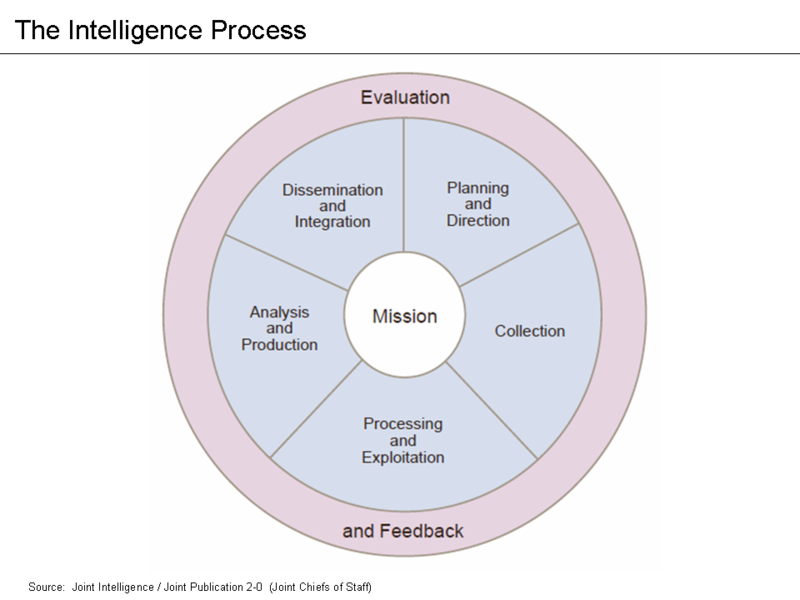
\includegraphics[width=0.5\linewidth]{800px-The_Intelligence_Process_JP_2-0.png}
\end{figure}
\subsection{Podaci, informacije i obaveštajni podaci}
U prethodnom delu se nismo pozabavili distinkcijom između ova tri pojma, što ćemo sada učiniti.\newline

{\bf Podaci} predstavljaju skup činjenica bez ikakvog objašnjenja ili analize i njih dobijamo tokom faze prikupljanja. Na osnovu svog formata se mogu klasifikovati u tri klase: struktuirani podaci (SQL baze), polustruktuirani podaci (JSON, XML i HTML dokumenti) i nestruktuirani podaci (tekst, artikli, blogovi, slike, videi itd.).\newline

{\bf Informacije} predstavljaju rezultat faze obrade. Dobijaju se obradom prikupljenih podataka. Zavisno od prirode podataka, obrada uključuje prevođenje, dešifrovanje ili izmenu formata, dodatno filtriranje, povezivanje, klasifikovanje, klasterovanje, itd. (na primer, svaki tekst koji sadrži neku reč)\newline

{\bf Obaveštajni podaci} su informacije koje su prikupljene, analizirane i interpretirane kako bi se podržale odluke u vezi sa nacionalnom bezbednošću, vojnom strategijom, sprovođenjem zakona, poslovanjem ili drugim oblastima koje zahtevaju informisano donošenje odluka. \newline

Ugrubo govoreći, u OSINT istrazi, podaci se mogu klasifikovati u {\bf sedam kategorija}:\newline

{\bf 1. Pojedinac}: Nalazi se tiču svih relevantnih informacija o jednoj osobi (ime i prezime, adresa, finansijsko stanje, onlajn pseudonim, email adresa, društvene mreže)\newline

{\bf 2. Grupa ljudi}: Obično u policijskim istragama, fokus se stavlja na grupu ljudi, njihove odnose i interakcije.\newline

{\bf 3. Organizacija}: Za razliku od grupe, organizacije karakteriše uglavnom uniforman cilj i postojanje hijerarhije. Primeri su kompanije, institucije čak i države. Ovde od značaja mogu biti razni biznis dogovori, strateški planovi, zaposleni i mušterije.\newline

{\bf 4. Računarski sistemi}: Sve informacije jednog IT sistema, poput domena, postojećih  poddomena, korišćeni softver itd.\newline

{\bf 5. Događaj}: Informacije koje mogu ukazivati na neko dešavanje. Obično se ne eksplicira ako nije događaj za širu javnost, te se mora „čitati između redova“. To se može postići posmatranjem interakcija ljudi onlajn ili uživo.\newline

{\bf 6. Lokacije}: Fizičke adrese ili koordinate.\newline

{\bf 7. Objekti}: Sve što ne spada u ostale klase. Slike, videi npr.
\subsection{Alati i tehnike}
Čak i ako postavimo precizno pitanje i zadamo krajnje rešivi zadatak u prvoj fazi našeg istraživanja, odgovor će zahtevati prikupljanje, obradu i analizu ogromne količine javno dostupnih podataka. Iz ovog razloga se moramo osloniti na neki vid automatizacije (posebno u fazi prikupljanja) kroz korišćenje specifičnih tehnika i alata.\newline

Pre svega, moramo primetiti da se alati poprilično brzo menjaju. Postoje dva razloga zašto i oba su skorijeg datuma. Prvi je povlačenje nekoliko bitnih alata od strane njihovih vlasnika poput Bazzell-ovog skupa popularnih interaktivnih onlajn alata u junu 2019. godine (\textit{Michael Bazzel} je jedan od vodećih OSINT istraživača) zbog navodne zloupotrebe njegovih alata, kao i nestanak meta-pretraživača \textit{searx.me} zbog poteškoća u održavanju i problema sa zakonom. Drugi razlog je dinamična priroda društvenih mreža. Facebook i Instagram aktivno podrivaju korišćenje alata i tehnika vezanih za OSINT. Stoga blokiraju odgovarajuće veb usluge, redovno menjaju svoj izvorni kod i ograničavaju kapacitete koje koristi OSINT zajednica. Na primer, Instagram uključuje specijalno kodiranje znakova u izvorni kod svoje veb stranice kako bi otežao direktno izvlačenje URL-ova.\newline

Uprkos svim ovim teškoćama, postoje različiti pristupi za pregled alata i tehnika. \textit{\href{https://osintframework.com/}{OSINT Framework}} je najrazvijeniji resurs. Njegov cilj je laka identifikacija OSINT alata pogodnih za pretragu na osnovu specifičnih identifikatora. Organizovan je kao struktura stabla sa identifikatorima kao korenima i kandidatskim alatima kao listovima.
\subsection{Veb pretraživači}
Postoje četiri tipa pretraživača: klasični pretraživači (\textit{crawler-based search engines}), direktorijumi koje uređuju ljudi (\textit{human-powered directories}), hibridni pretraživači (\textit{hybrid search engines}) i meta pretraživači (\textit{meta search engines}).\newline

Za razliku od jednostavnih tekstualnih pretraga, specifično formulisanje upita za pretragu može značajno poboljšati rezultate. Stoga se unos u korisnički interfejs obogaćuje proširenim parametrima pretrage kombinovanim sa logičkim simbolima. Prošireni parametri pretrage su specijalni karakteri i komande koje značajno proširuju mogućnosti tekstualne pretrage. Primeri uključuju: upotrebu navodnika za zahtev za tačnim podudaranjem; termin \textit{intext:} za pretragu unutar tela ili dokumenta; termin \textit{inurl:} za termin u URL-u. Njihova upotreba proizvodi preciznije rezultate. Ova tehnika je prvi put primenjena u \textit{Google} pretraživaču i stoga je poznata kao \textit{Google Hacking} ili \textit{Dorking}.\newline

S obzirom na identifikatore kao što su korisnička imena, brojevi telefona ili e-mail adrese kao unose, rezultati opisanih veb pretraživača mogu biti ograničeni. Ovo takođe važi za analizu drugog potencijalno relevantnog sadržaja kao što su slike ili lokacije. Specijalizovani pretraživači su u stanju da adresiraju takve vrste unosa. Neki od specijalzovanih pretraživača su: pretraživači za pretragu slika (\textit{\href{https://images.google.com/}{Google Images}}), pretraživači za pretrage korisničkih imena (\textit{\href{https://whatsmyname.app/}{ WhatsMyName}}), pretraživači za e-mail adrese (\textit{\href{https://thatsthem.com/}{ThatsThem}}), pretraživači za lokacije (\textit{\href{https://earth.google.com/web/}{Google Earth}}) ili pretraživači za brojeve telefone (\textit{\href{https://whocalld.com/}}{Whocalld}}).\newline

Drugi manje poznati, ali takođe zanimljivi specijalizovani pretraživači: dokumentovanih imena (\textit{\href{https://namesdir.com/}{Names Directory}}), vesti (\textit{\href{https://news.google.com}{Google News}}), naučnih radova (\textit{\href{https://sci-hub.se/}{Sci-Hub}}), sigurnosnih ranjivosti (\textit{\href{https://cve.mitre.org/}{Common Vulnerabilities and Exposures}}), resursa povezanih na internet (\textit{\href{https://www.shodan.io/}{Shodan}}).
\subsection{Društvene mreže}
Obećavajući izvori informacija o pojedincima ili grupama ljudi su društvene mreže kao što su Facebook, Instagram, LinkedIn, Twitter, Pinterest, YouTube, pa čak i PayPal, gde ljudi dele lične informacije i komuniciraju sa porodicom, prijateljima, kolegama ili čak nepoznatim osobama.\newline

Detaljna analiza je podržana automatskim alatima za preuzimanje prilagođenim odgovarajućoj društvenoj mreži, na primer \textit{InstaLooter} i \textit{Instaloader}, fokusiranim na Instagram ili \textit{TweetBeaver} i \textit{exportdata} fokusiranim na Twitter.\newline

Pored toga, postoji veliki broj aplikacija, ekstenzija za pregledače ili veb usluga specijalizovanih za različite društvene mreže koje nude ekstrakciju određenih informacija ili pripremu za manipulaciju URL-ovima (npr. ekstrakcija Facebook userID-a \textit{Facebook UserID LookUp}) ili samostalne informacije (npr. prikazivanje promena biografije na Twitter-u \textit{Twitter Biography Changes}). Izazovi se javljaju jer neke društvene mreže omogućavaju primenu jakih privatnih podešavanja na profilu što sprečava detaljan pregled. Iako ovo isključuje značajnu količinu informacija, to ne sprečava nužno curenje informacija. Na primer, moguće je identifikovati javne objave koje nisu direktno prikazane na stranici privatnog profila (\textit{\href{https://www.osintcurio.us/}{OSINT Curious}}). Druga opcija je analiza povezanih naloga koji mogu biti javni i otkrivati informacije o cilju.\newline

Alati i tehnike za pretragu na društvenim mrežama se stalno razvijaju. Kao što je ranije pomenuto, ovo je uzrokovano čestim promenama samih društvenih mreža kako bi se sprečila eksploatacija informacija na načine koji nisu prvobitno predviđeni. Značajan primer je nestanak Facebook-ove graf pretrage. Funkcionisala je tako što je korisnicima omogućavala da koriste govorni jezik za postavljanje pitanja i pretragu unutar društvene mreže, čineći pretragu informacija mnogo interaktivnijom i detaljnijom nego standardna pretraga ključnih reči. Prvobitno uvedena za opštu upotrebu, nudila je moćan pristup za dobijanje informacija. Ovo se promenilo 2014. godine, a funkcionalnost graf pretrage bila je dostupna samo pomoću modifikacija URL-ova. Na kraju, svi alati i tehnike koje su se oslanjale na graf pretragu prestali su da rade sredinom 2019. godine.\newpage
\section{Odgovor društva}
Cilj svake OSINT istrage je da se prikupe informacije o meti. Međutim, ovo može biti u suprotnosti sa interesima mete. Iz perspektive istog, otkrivanje informacija može biti nepoželjno jer narušava privatnost, ili čak štetno ako se rezultati iskoriste protiv mete u kriminalnom aktu. Ovo postavlja pitanje da li postoje mere za sprečavanje eksploatacije podataka.
\subsection{Protivmere}
Suočeni sa neželjenim otkrivanjem ličnih podataka, validno je pitanje šta svako može učiniti da smanji količinu kritičnih informacija. Odgovor leži u principu da se podaci čuvaju privatno i da se deli što manje informacija. Što je manje javno dostupnih podataka o pojedincu, to je manji rizik od otkrivanja tokom OSINT istrage. Takođe postoje neke dobre prakse vremenom ustanovljene.\newline

Prva preporuka je sticanje što većeg uvida u svoje aktivnosti na društvenim mrežama i aktivno smanjenje količine deljenih informacija. Najefikasnija strategija bi bila potpuno izbegavanje učešća na društvenim mrežama i zatvaranje svih postojećih naloga. Međutim, interakcije na društvenim mrežama su neophodne u svakodnevnom životu. Preporučuje se prilagođavanje podešavanja privatnosti svih profila. Ovo može uključivati korišćenje pseudonima umesto pravog imena. Pored toga, čak i sa strogim podešavanjima privatnosti, pametno je tretirati sve deljene informacije kao javno dostupne i izbegavati izlaganje sadržaja neprikladnog za široku publiku ili kompromitujućeg u pogrešnim rukama.\newline

Pored pregleda aktivnosti na društvenim mrežama, još jedan savet je izbegavanje objavljivanja ličnih informacija kao što su kućna adresa, broj telefona ili email adresa. U slučaju da je objavljivanje neophodno zbog poslovnih razloga, izvodljiv pristup je postavljanje odvojenih kontakt informacija.
\subsection{Pravni okvir}
Sa porastom problema izazvanih sve većim opštim prisustvom na internetu, brojne institucije su se odlučile na proces pravne regularizacije OSINT metoda. Navešćemo par primera. \newline \newline
  \indent \textbf{GDPR}: 2016.Evropska unija je uvela Opštu uredbu o zaštiti podataka (\textit{GDPR}). Ova uredba uvodi mere zaštite ličnih podataka fizičkih lica. Na primer, zahteva obaveštenje ako se prikupljaju lični podaci i saglasnost za obradu ličnih podataka. Fokusirajući se na OSINT istrage pojedinaca, primena ove uredbe bi ozbiljno ograničila bilo koje prikupljanje ili obradu podataka.\newpage

\textbf{Države}: Navešćemo samo primer Nemačke koja se kroz odluku Saveznog suda Nemačke još 2008. obračunala sa svim OSINT pretragama, legalizujući ih, smatrajući javno dostupne informacije legalnim za opšte čitanje.
Sa uvođenjem GDPR-a 2016. godine, obrada ličnih podataka je dodatno regulisana. Ovo se takođe primenjuje u slučaju da istragu sprovode organi za sprovođenje zakona sa direktivom EU 2016/680 koja posebno adresira zaštitu fizičkih lica u vezi sa obradom ličnih podataka od strane nadležnih organa u svrhe sprečavanja, istrage, otkrivanja ili gonjenja krivičnih dela ili izvršenja krivičnih sankcija.
Pored toga, prikupljanje javnih informacija od strane vlasti predmet je kontroverznih rasprava. Dok su ciljne pretrage pokrivene opštim ovlašćenjima, korišćenje široko baziranih OSINT pretraga (npr. Big Data) je sporno.\newline

\textbf{Uslovi korišćenja usluga}: Implicirano je da se podaci prikupljeni sa društvenih mreža mogu smatrati javnim. Međutim, pristup najčešćim društvenim mrežama kao što su Facebook ili Instagram je ograničen registracionim procesom. To znači da samo registrovani članovi te društvene mreže imaju pravo pristupa. Iako je ova registracija besplatna, zahteva ulazak u ugovor sa društvenom mrežom. Tako, korisnik mora da pristane na uslove korišćenja te društvene mreže. U nekim slučajevima, primena OSINT alata i tehnika krši ovaj ugovor. Na primer, zabranjeno je pristupanje Facebook-u ili Instagram-u na automatizovan način prema njihovim uslovima korišćenja ili stvaranje Facebook naloga koristeći lažno ime.
\subsection{Etička pitanja}
U pogledu etičke perspektive, takođe je potrebno diskutovati da li etička upotreba informacija zavisi od toga da li su te informacije namerno učinjene javnim. Na primer, u PayPal-u je moguće pretražiti listu korisnika PayPal-a samo pružanjem nekoliko karaktera imena. Često odgovarajući profili uključuju dodatne informacije kao što je trenutni grad prebivališta. Većina ljudi je dala svoje ime verujući da će samo ograničeni broj ljudi imati pristup tim informacijama. Shodno tome, većina korisnika nije svesna da se neki od njihovih podataka može smatrati javno dostupnim.\newline

Podaci o proboju često se objavljuju, bilo da se naglasi zahtev za uzimanje podataka ili se dokaže uspešan napad. S obzirom na to da su takvi podaci javno dostupni i veoma vredni, OSINT istraživači se pitaju da li se oni mogu iskoristiti za istragu. Po ovom pitanju, mišljenja se razlikuju. Za neke je upotreba neetička jer podaci nikada nisu bili namenjeni za javnost i dobijeni su putem kriminalnih dela. Za druge, nije bitno kako su dobijeni, i oni dopunjuju svoju zbirku podataka.\newpage
\section{Zaključak}
Osnovne mere za zaštitu privatnih informacija od izloženosti OSINT istragama su dostupne, ali nisu uvek vrlo praktične. U celini, upotreba javnih podataka je (u većini slučajeva) zakonita, omogućavajući OSINT istrage fokusirane na računarske sisteme, objekte ili lokacije. Situacija za OSINT istrage o pojedincima je drugačija jer takve istrage zavise od prikupljanja i obrade ličnih podataka. Takvi tipovi podataka podležu ograničenjima na evropskom nivou, što čini pravni status OSINT-a fokusiranog na fizička lica, barem od strane nevladinih entiteta, neizvesnim i predmetom daljih pojašnjenja. Sa etičkog stanovišta, može se primetiti da nije sve što je tehnički moguće i moralno opravdano.
\newpage
\section{Literatura}
\begin{enumerate}[label=(\arabic*)]
\item \url{https://www.dni.gov/files/documents/IC_Consumers_Guide_2011.pdf}
\item \url{https://www.bellingcat.com/resources/articles/2016/07/14/a-brief-history-of-open-source-intelligence/ }
\item \url{https://www.bellingcat.com/}
\item \url{https://www.europol.europa.eu/stopchldabuse}
\item \url{https://www.sfgate.com/news/article/Vast-search-off-coast-for-data-wizard-2620302.php}
\item
\url{https://www.bbc.com/news/world-europe-37538453}
\item Gibson H, in Open Source Intelligence Investigation – From Strategy to Implementation, ed. by B. Akhgar,
P.S. Bayerl, F. Sampson (Springer, 2016), 69 – 93
\item \url{https://osintframework.com/}
\item
\url{https://en.wikipedia.org/wiki/Intelligence_cycle}
\item
\url{https://en.wikipedia.org/wiki/Open-source_intelligence}
\end{enumerate}
\end{document} 
